\documentclass{article}
\usepackage{hyperref}
\usepackage{palatino}
\usepackage{amsmath}
\usepackage{amsthm}
\usepackage{setspace}

\newtheorem*{theorem}{Theorem}

\newcommand{\summary}[1]{
\renewcommand{\maketitle}{{%
\flushleft\textsf{Ben Greenman \hfill \today} \\
\textsf{\hfill #1} \\
\vspace{1mm}
\hrule
\vspace{0.4cm}}}
\maketitle
}

\newcommand{\swtable}[2]{
\vspace{0.5cm}
\subsubsection*{Strengths}
\begin{itemize}
#1
\end{itemize}
\vspace{0.1cm}

\vspace{0.5cm}
\subsubsection*{Weaknesses}
\begin{itemize}
#2
\end{itemize}
\vspace{0.1cm}
}

\newcommand{\questions}[1]{
\vspace{0.5cm}
\subsubsection*{Questions}
\begin{itemize}
#1
\end{itemize}
\vspace{0.1cm}
}
\newcommand{\comments}[1]{
\vspace{0.5cm}
\subsubsection*{Comments}
\begin{itemize}
#1
\end{itemize}
\vspace{0.1cm}
}


\begin{document}
\maketitle

\begin{abstract}
Craig Interpolants: definitions, intuitions, and applications.
\end{abstract}

%% -----------------------------------------------------------------------------
\section{Definitions}

The following sentences $A$, $B$, $C$ are special.
For each, $A$ implies $B$.
Furthermore, $A$ implies $C$ and $C$ implies $B$.

\begin{itemize}
\item[]
  \begin{itemize}
  \item[]
    $\begin{array}{l l l}
      A & = & \neg(P \wedge Q) \Rightarrow (\neg R \wedge Q)
    \\B & = & (T \Rightarrow P) \wedge (T \Rightarrow \neg R)
    \\C & = & (P \vee \neg R)
    \end{array}$
  \end{itemize}
\item[]
  \begin{itemize}
  \item[]
    $\begin{array}{l l l}
      A & = & P \vee (Q \wedge R)
    \\B & = & P \vee \neg\neg Q
    \\C & = & P \vee Q
    \end{array}$
  \end{itemize}
\item[]
  \begin{itemize}
  \item[]
    $\begin{array}{l l l}
      A & = & \neg(P \wedge Q) \implies (\neg R \wedge Q)
    \\B & = & (S \Rightarrow P) \vee (S \Rightarrow \neg R)
    \\C & = & P \vee \neg R
    \end{array}$
  \end{itemize}
\end{itemize}



\begin{defn}
  Craig Interpolant (1957) \\
  Suppose $A$ and $B$ are logical formulas.
  An interpolant $C$ for the pair $(A, B)$ is:
  \begin{itemize}
  \item Implied by $A$: $\vdash A \Rightarrow C$
  \item Sufficient to prove $B$: $\vdash C \Rightarrow B$
  \item Expressed over the common variables of $A$ and $B$:
  \subitem $\fvs{C} \subseteq \fvs{A} \cup \fvs{B}$
  \end{itemize}
\end{defn}
\begin{theorem}
  If $\vdash A \Rightarrow B$ then an interpolant for $(A, B)$ exists~\cite{c-jsl-1957}.
\end{theorem}
\begin{proof}
  By induction on the size of $V = \fvs{A} \setminus \fvs{B}$.
  If $V$ is empty, $A$ is an interpolant.
  Else choose any variable $v \in V$ and define $A' = A[\top/v] \vee A[\bot/v]$.
  By the induction hypothesis, an interpolant for $(A', B)$ is an interpolant for $(A, B)$.

  If $\fvs{A} \cap \fvs{B} = \emptyset$ then either $\vdash \neg A$ or $\vdash B$.
\end{proof}

\begin{challenge}
Find an optimal interpolant for $(A, B)$ i.e. smallest, least variables, quantifier-free.
\end{challenge}
The proof above can make an exponentially large term.
Craig's proof introduces quantifiers.


%% -----------------------------------------------------------------------------
\section{Craig Interpolants in Model Checking}

Very simple program:
\begin{lstlisting}
void f(int n) {
    int x = n;
    int y = n + 1;
    assert(y == x + 1);
}
\end{lstlisting}

Goal: prove that the assertion on line 4 is never violated.

At line 4, we have the following premise ($A$) and goal ($B$):

$$\begin{array}{l l l}
  A & = & \{n \in {\tt short} \wedge x = n \wedge y = n + 1 \}
\\B & = & y = x + 1
\end{array}$$

A suitable interpolant for $(A, B)$ is $B$.


\subsection{Basic Strategy}
Start by finding a path in the program to as {\tt assert} statement.
The path will be represented by primarily by transitions $T(s_i, s_j)$ from
 one state $s_i$ to a successor state $s_j$.
% TODO c?
The final state in the path is the assertion $C$ we wish to prove correct;
 in total we can represent the path as a formula:
 $$p = T(s_0, s_1) \wedge T(s_1, s_2) \wedge \ldots \wedge T(s_{n-1}, s_n) \wedge C(s_n)$$
The formula should be true of a specific path, but we want to know whether it
 holds for all paths.
The key idea of interpolation-based model checking is to use our proof that $p$
 is correct to find counterexamples to $C$.

We take the (false) formula $p'$:
 $$p' = T(s_0, s_1) \wedge T(s_1, s_2) \wedge \ldots \wedge T(s_{n-1}, s_n) \wedge \neg C(s_n)$$
 and consider of each $\wedge$ from left to right in turn as a formula $A \wedge B$
 where $A$ and $B$ are mutually inconsistent.
Then we apply interpolation to get a formula $A'$ that is:
\begin{itemize}
\item Implied by $A$
\item Inconsistent with $B$
\item Expressed over the common atoms: $\fvs{A} \setminus \fvs{B}$
\end{itemize}

A good interpolant $A'$ will contain no irrelevant information about $B$.
In other words, $A'$ contains only the facts about $A$ necessary to prove the
 assertion $C$ holds later in the path.


\subsubsection{Equivalent Definitions}
Note: this definition is classically equal to Craig's original, just switch $\neg B$ for $B$.
It is also more common in the model-checking community~\cite{m-tacas-2005}.
Here are a few new-style interpolants.

\begin{itemize}
\item[]
  \begin{itemize}
  \item[]
    $\begin{array}{l l l}
      A & = & u = x \wedge f(u, y) = z
    \\B & = & v = y \wedge f(x, v) \neq z
    \\C & = & f(x,y) = z
    \end{array}$
  \end{itemize}
\item[]
  \begin{itemize}
  \item[]
    $\begin{array}{l l l}
      A & = & x \leq y \wedge y \leq z
    \\B & = & x - z - 1 \geq 0
    \\C & = & x \leq z
    \end{array}$
  \end{itemize}
\end{itemize}


\subsection{While Programs}

Take a small while program~\cite{bkrw-preprint-2010}:

\begin{lstlisting}
  int i = 0;
  while (i < 1000)
    i += 1;
  assert(i <= 1000);
\end{lstlisting}

Using interpolation,\footnote{Also: bounded model checking, predicate abstraction, and lazy abstraction.} we can prove that the assertion on line 4 never fails.

First, the control-flow-graph of our program is:

\begin{center}
  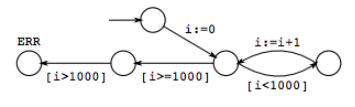
\includegraphics[scale=0.6]{src/example-cfg.png}
\end{center}

By unrolling the program, exploring paths, and computing interpolants for
 each state (by splitting the path formula into two inconsistent conjunctions) we get the tree:

\begin{center}
  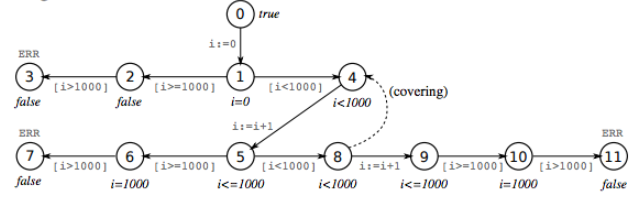
\includegraphics[scale=0.5]{src/example-tree.png}
\end{center}

Correctness follows because the 3 error states are unreachable and state 4 \emph{covers}
 state 8.
The covering condition follows because states 4 and 8 refer to the same control-flow
 condition and the proposition $i < 1000$ at state 8 implies the proposition at
 state 4.

\subsection{More Examples}

From D'Silva~\cite{d-nyu-2015}:

\begin{lstlisting}
void g(int i, int j) {
  int x = i;
  int y = j;
  int tmp;
  while (*) {
    tmp = x;
    x = y + 1;
    y = tmp + 1;
  }
  if (i == j && x <= 10) {
    assert(y <= 10);
  }
}
\end{lstlisting}

A few possible interpolants:
\begin{enumerate}
\item $i = j \implies x \le y$
\item $i = j \implies y \le x$
\item $(1) \wedge (2) \implies x = y$
\end{enumerate}


%% -----------------------------------------------------------------------------
\section{Alternative: Image Computation}
% image computation = compute successors

Before interpolation, ``the way'' to annotate states was \emph{image computation}
 i.e. computing all successors of each state~\cite{m-tacas-2005}.
One would compute the strongest invariant of a program with initial state $I$
 and transition relation $T$ by taking the fixed point of all strongest
 postconditions at each reachable state.

 $$R(I, T) = \mu U.\, I \vee \mathsf{post}_T(Q)$$

Each $\mathsf{post}_T(Q)$ for a state formula $Q$ is easy to express in
 propositional logic, but difficult to compute:

  $$\mathsf{post}_T(Q) = \exists S .\, Q \wedge T$$
 where $S$ is a signature representing the entire state space.
At least we know how to compute it, but the process is very slow for all
 but the smallest programs.
If $\mathsf{post}_T$ is monotonic, the least fixed point of $Q$ exists
 and is the strongest invariant of the program.\footnote{Other fixed points
  are inductive invariants of the program.}


%% -----------------------------------------------------------------------------
\section{How to Derive Interpolants}

Core idea for how to derive an interpolant from a refutation of $A \wedge B$.

\subsection{Basic Logic}

Start with a quantifier-free propositional logic and these rules
 for proving $\not\vdash A \wedge B$~\cite{d-nyu-2015}.
Very important to divide rules based on where the variables occur.

\begin{mathpar}
  \inferrule*[left=A-Hyp]{
    C \in A
  }{
    \vdash C
  }

  \inferrule*[left=A-Res]{
    x \in \fvs{A} \setminus \fvs{B}
    \\
    \vdash C \vee x 
    \\
    \vdash \neg x \vee D
  }{
    \vdash C \vee D
  }

  \inferrule*[left=B-Hyp]{
    C \in B
  }{
    \vdash C
  }

  \inferrule*[left=B-Res]{
    x \in \fvs{B}
    \\
    \vdash C \vee x
    \\
    \vdash \neg x \vee D
  }{
    \vdash C \vee D
  }
\end{mathpar}

Then annotate rules with \emph{partial interpolants}.

\begin{mathpar}
  \inferrule*[left=A-Hyp]{
    C \in A
  }{
    \vdash C ~~~ [\{\, C' \in C \mid \fvs{C'} \subseteq \fvs{B} \,\}]
  }

  \inferrule*[left=A-Res]{
    x \in \fvs{A} \setminus \fvs{B}
    \\
    \vdash C \vee x ~~~ [I_1]
    \\
    \vdash \neg x \vee D ~~~ [I_2]
  }{
    \vdash C \vee D ~~~ [I_1 \vee I_2]
  }

  \inferrule*[left=B-Hyp]{
    C \in B
  }{
    \vdash C ~~~ [\top]
  }

  \inferrule*[left=B-Res]{
    x \in \fvs{B}
    \\
    \vdash C \vee x ~~~ [I_1]
    \\
    \vdash \neg x \vee D ~~~ [I_2]
  }{
    \vdash C \vee D ~~~ [I_1 \wedge I_2]
  }
\end{mathpar}


\subsubsection{Sample Proof}

$$\begin{array}{l l l}
  A & = & (a_1 \vee \neg a_2) \wedge (\neg a_1 \vee \neg a_3) \wedge a_2
\\B & = & (\neg a_2 \vee a_3) \wedge (a_2 \vee a_4) \wedge \neg a_4
\end{array}$$

An interpolant is $C = \neg a_3 \wedge a_2$, derived below:
\vspace{0.2cm}

\hbox{\hspace{-3cm}\begin{mathpar}
  \inferrule*{
    \inferrule*{
      \inferrule*{
        \inferrule*{
        }{
          a_1 \vee \neg a_2 [\neg a_2]
        }
        \\
        \inferrule*{
        }{
          \neg a_1 \vee \neg a_3 ~~~ [\neg a_3]
        }
      }{
        \neg a_2 \vee \neg a_3 ~~~ [\neg a_2 \vee \neg a_3]
      }
      \\
      \inferrule*{
      }{
        a_2 ~~~ [a_2]
      }
    }{
      \neg a_3 ~~~ [\neg a_3 \wedge a_2]
    }
    \\\\
    \inferrule*{
      \inferrule*{
      }{
        \neg a_2 \vee a_3 ~~~ [\top]
      }
      \\\\
      \inferrule*{
        a_2 \vee a_4 ~~~ [\top]
        \\
        \neg a_4 ~~~ [\top]
      }{
        a_2 ~~~ [\top]
      }
    }{
      a_3 ~~~ [\top]
    }
  }{
    \vdash \bot ~~~ [\neg a_3 \wedge a_2]
  }
\end{mathpar}}


\newpage
\subsection{Basic Arithmetic}

McMillan's simple rules for linear inequalities~\cite{m-tcs-2005}:

\begin{mathpar}
  \inferrule*[left=H$<$A]{
    0 \leq x \in A
  }{
    \vdash 0 \leq x ~~~ [x]
  }

  \inferrule*[left=H$<$B]{
    0 \leq x \in B
  }{
    \vdash 0 \leq x ~~~ [\top]
  }

  \inferrule*[left=Comb]{
    \vdash 0 \leq y - x ~~~ [y - x]
    \\\\
    \vdash 0 \leq z - y ~~~ [z - y]
  }{
    \vdash 0 \leq c_1x + c_2y ~~~ [c_1 x' + c_2 y']
  }
\end{mathpar}

\subsubsection{Example}

$$\begin{array}{l l l}
  A & = & (0 \leq y - x) \wedge (0 \leq z - y)
\\B & = & 0 \leq x - z - 1
\end{array}$$

Now we show that $A$ and $B$ are inconsistent and derive an interpolant.

\vspace{0.2cm}

\begin{mathpar}
  \inferrule*{
    \inferrule*{
      \inferrule*{
      }{
        \vdash 0 \leq y - x ~~~ [y - x]
      }
      \\
      \inferrule*{
      }{
        \vdash 0 \leq z - x ~~~ [z - y]
      }
    }{
      \vdash 0 \leq z - x ~~~ [z - x]
    }
    \\
    \inferrule*{
    }{
      \vdash 0 \leq x - z - 1 ~~~ [\top]
    }
  }{
    \vdash 0 \leq -1 ~~~ [z - x]
  }
\end{mathpar}


\subsection{Complexity Results}
At least one of the following is true~\cite{m-pal-1984}:
\begin{itemize}
\item $\mathsf{P} = \mathsf{NP}$
\item $\mathsf{NP} \neq \mathsf{coNP}$
\item Then interpolants in propositional logic are not in general computable
      in time polynomial in the size of $(A, B)$.
\end{itemize}

% Also by Pudl\'{a}k
If the propositional formula $A \wedge B$
 has a refutation of size $n$ there
 is an interpolant of circuit size $3n$~\cite{k-jsl-1997}.
% circuit size = num gates?

%% -----------------------------------------------------------------------------
\section{Applications of Craig Interpolation in Model Checking}
McMillan~\cite{m-tacas-2005} gives three examples of using interpolants to do
 model checking faster / more efficiently.
\begin{enumerate}
\item Find invariants of program paths
\item Choose predicates to approximate a program state.
      Relies on interpolants not introducting new quantifiers.% Predicate Abstraction
\item Filter irrelevant details from a transition relation % 'based on symmetric interp'
\end{enumerate}


%% -----------------------------------------------------------------------------
\section{Theories with Efficient Interpolants}
\begin{itemize}
\item Resolution, bounded arithmetic theory, linear equational calculus, cutting planes~\cite{k-jsl-1997}.
\item Linear Arithmetic with quantifiers ($\mathsf{LA(Q)}$)~\cite{m-tcs-2005}.
\item Datatype theories~\cite{kmz-sigsoft-2006}.
\item Quatifier-free, linear inequalities, equality, uninterpreted functions~\cite{m-tcs-2005}.
% http://www.kenmcmil.com/pubs/TCS05.pdf
\item Quantifier-free Presburger Arithmetic with arrays~\cite{bkrw-preprint-2010}.
\item $\mathsf{DL(Q)}, \mathsf{UTVPI}$
\item
  Linear Diophantine \& Linear Modular equations~\cite{jcg-cav-2008}
  % dioph = polynomial, integer solutions, 2+ unknowns
\item Bit vectors~\cite{g-fmcad-2011}.
\end{itemize}

%% -----------------------------------------------------------------------------
\section{Reflecting}

\begin{quote}
  "Craig's Theorem is about the last significant property of first-order logic
   that has come to light. Is there something deeper going on here, and if so,
   can we prove it?" - Van Bentham, 2008
\end{quote}

%% -----------------------------------------------------------------------------
\vfill{}
\footnotesize
\bibliographystyle{plain}
\bibliography{interp}

\newpage
\section*{Appendix: Craig's Statement \& Proof}

\hspace{-2cm}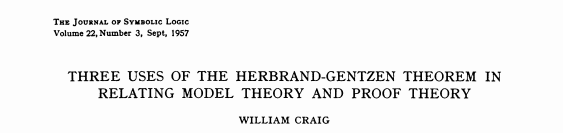
\includegraphics[scale=0.7]{src/c0.png}

\hspace{-2.4cm}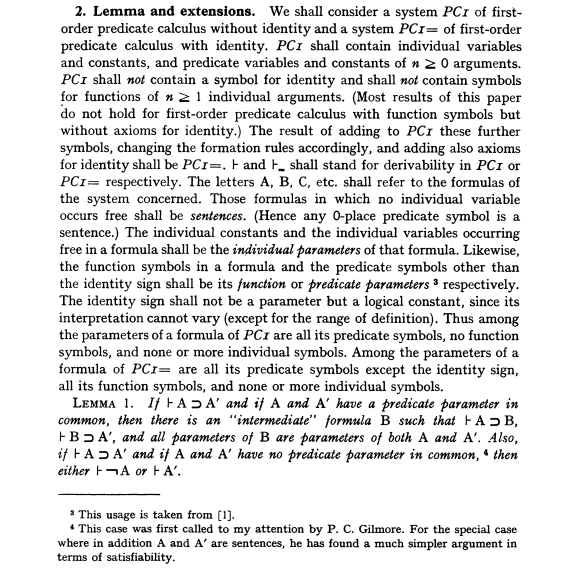
\includegraphics[scale=0.7]{src/c2.png}

\hspace{-2cm}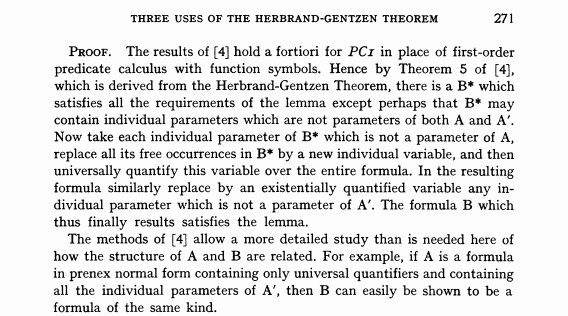
\includegraphics[scale=0.7]{src/c3.png}



\end{document}
